\section{Hiện thực Firmware và Software}

    \subsection{Kiến trúc phần mềm}

        \begin{figure}[H]
            \centering
            \begin{minipage}[t]{0.48\textwidth}
                \centering
                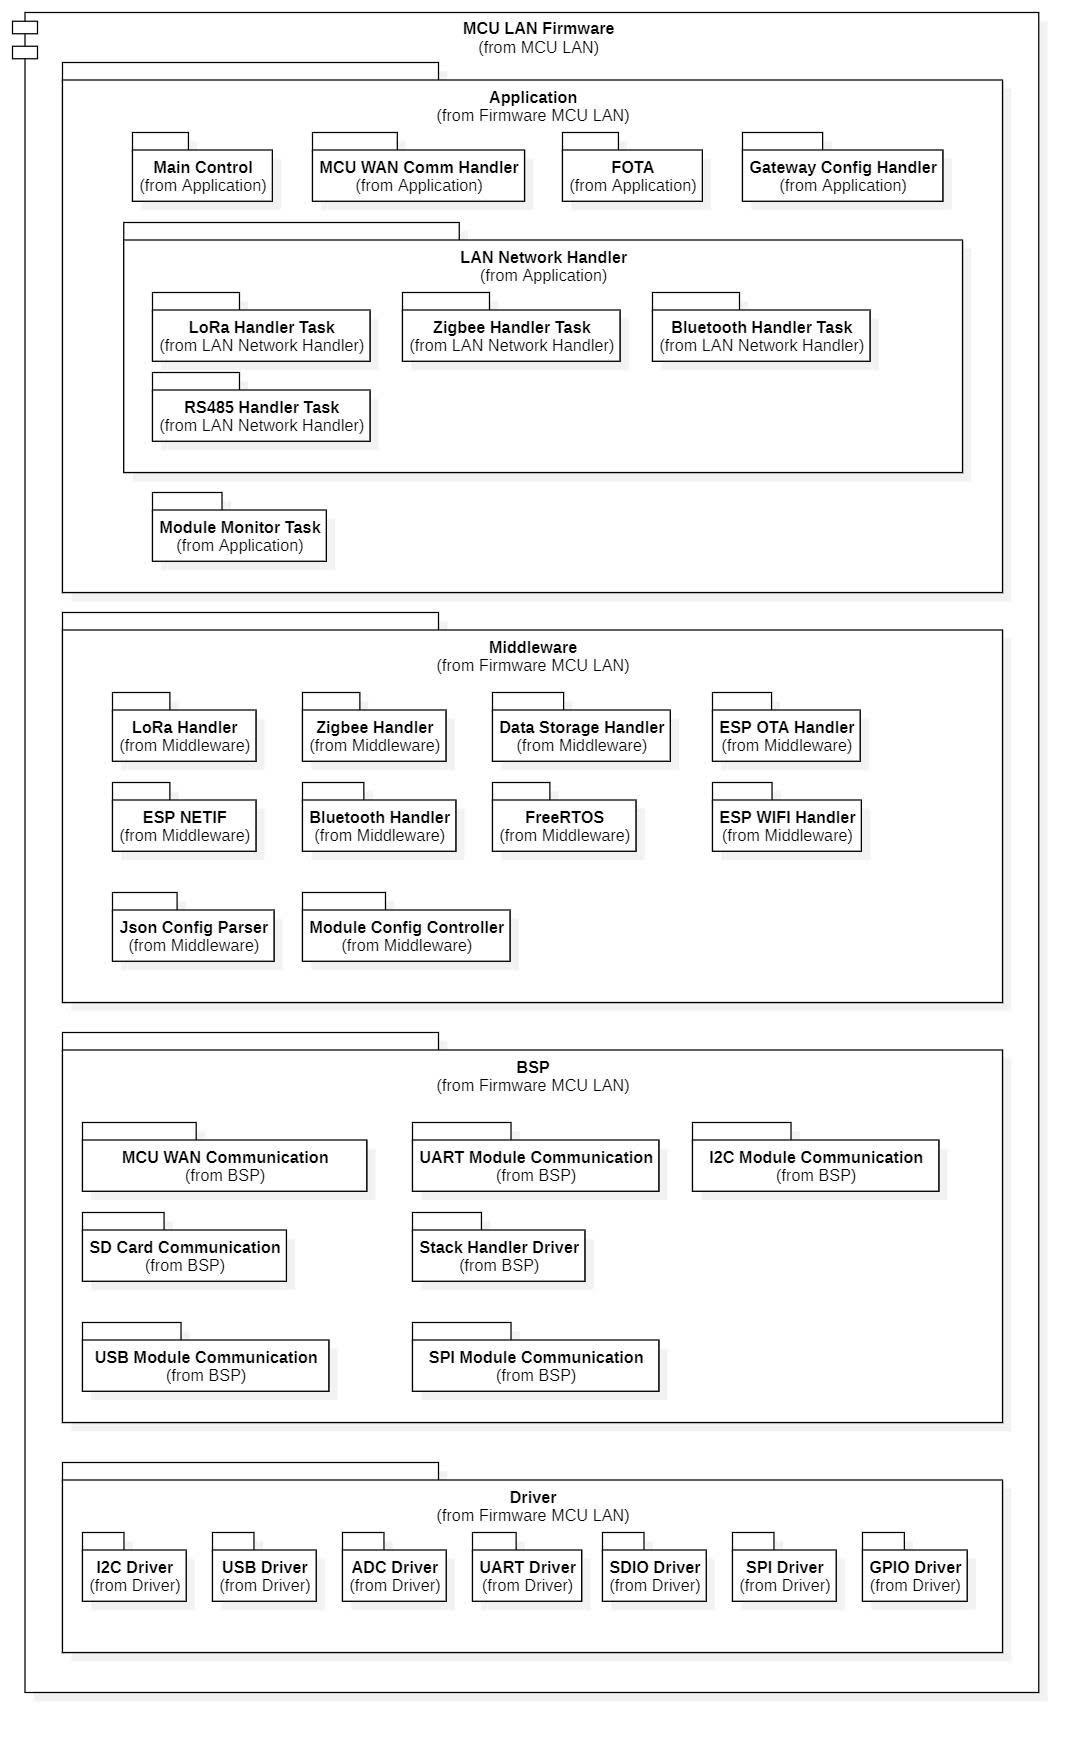
\includegraphics[width=\textwidth]{figures/DATN/design_mculanfirmware.jpg}
                \caption{MCU LAN Firmware}
                \label{fig:mculan_firmware}
            \end{minipage}
            % \hfill
            \begin{minipage}[t]{0.48\textwidth}
                \centering
                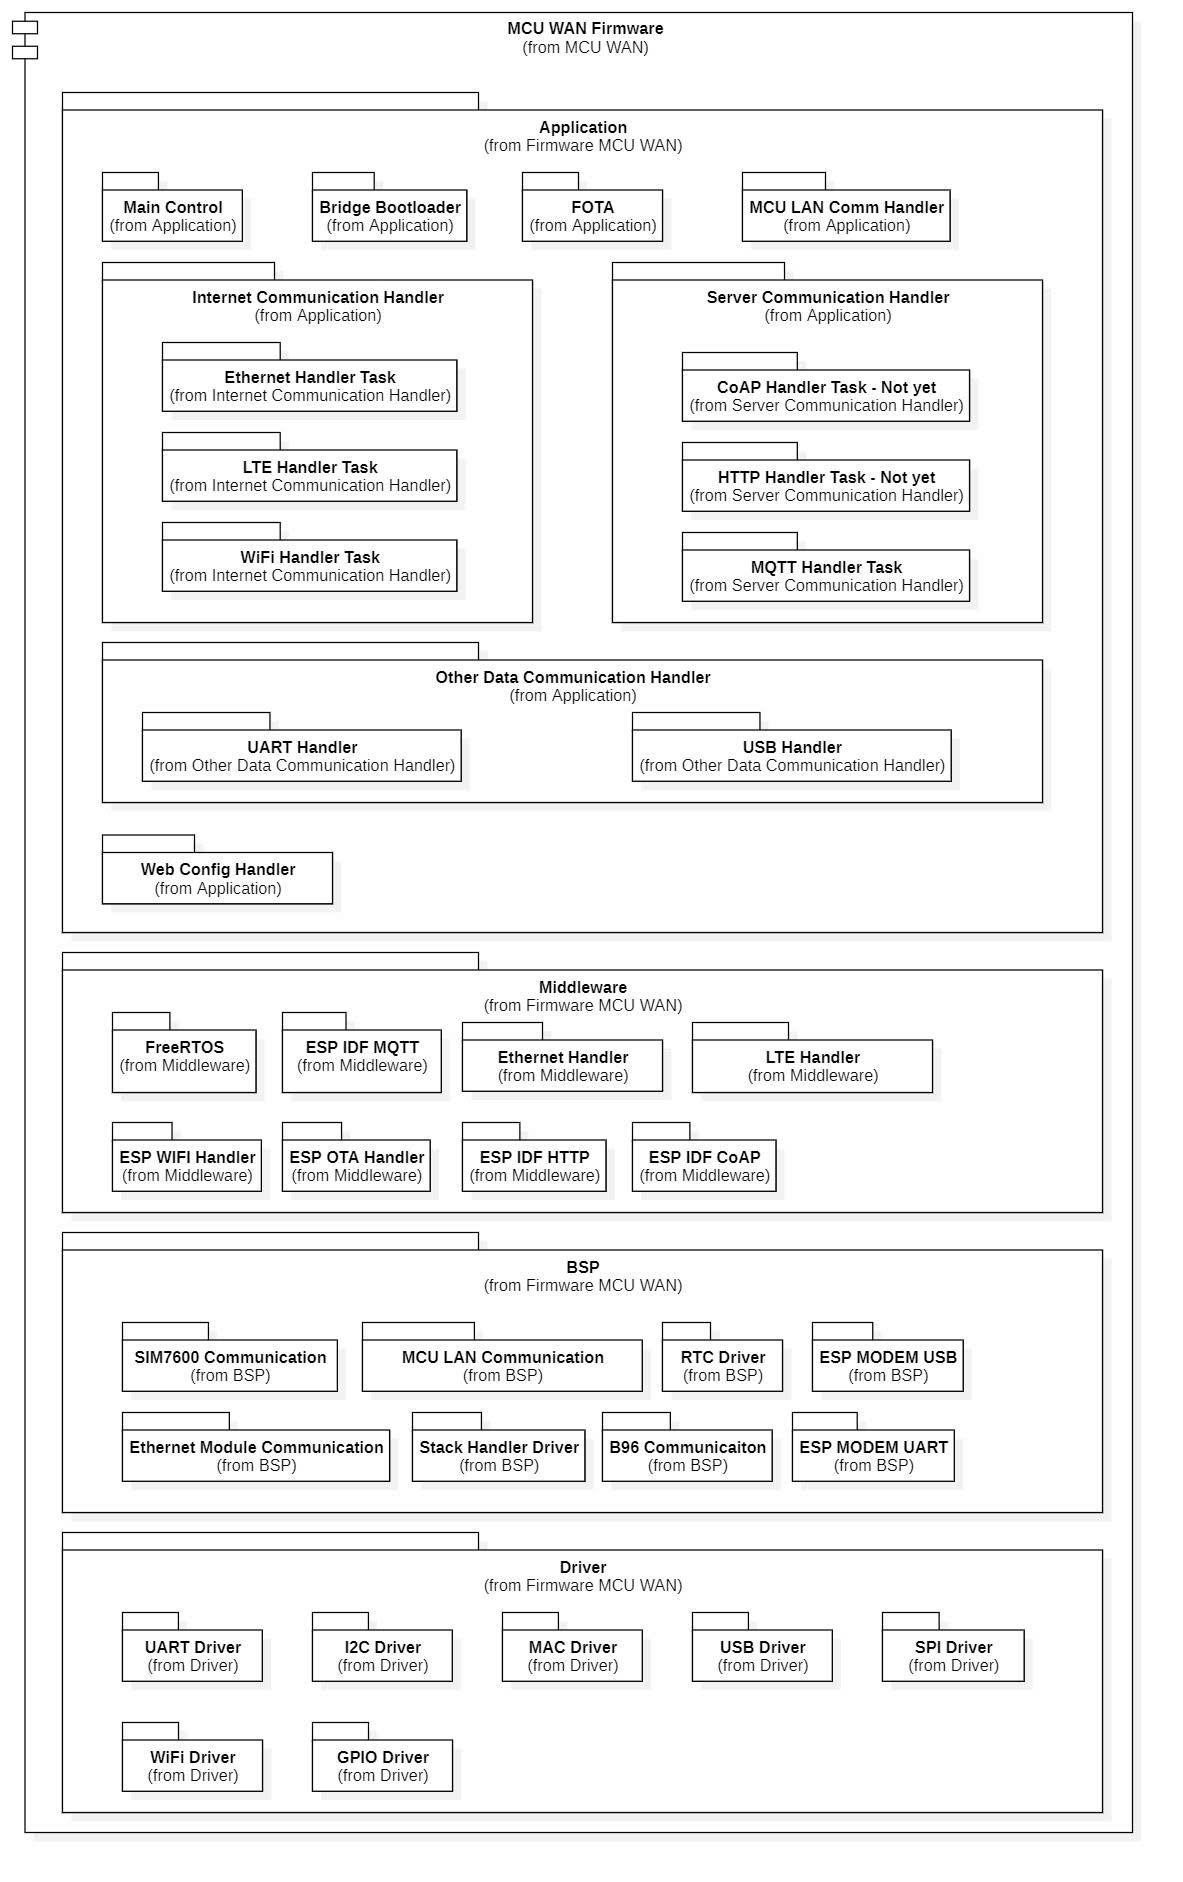
\includegraphics[width=\textwidth]{figures/DATN/design_mcuwanfirmware.jpg}
                \caption{MCU WAN Firmware}
                \label{fig:mcuwan_firmware}
            \end{minipage}
        \end{figure}
        
        Phần mềm được xây dựng trên nền tảng FreeRTOS với cấu trúc phân lớp chuẩn hóa gồm Application, Middleware, BSP và Driver. Kiến trúc này tách hệ thống thành hai miền xử lý độc lập theo mô hình Dual-MCU Master--Slave, vừa tối ưu tài nguyên vừa đảm bảo tính module hóa cho các giao thức mở rộng.

        Trong đó, LAN-MCU đóng vai trò điều phối lớp dưới, trực tiếp quản lý các kết nối nội bộ như LoRa, Zigbee, BLE và RS-485. Nhiệm vụ trọng tâm của LAN-MCU là thu thập, kiểm chứng và chuẩn hóa dữ liệu thô từ sensor trước khi đẩy lên kênh truyền thông nội bộ.
        
        Ngược lại, WAN-MCU đảm nhiệm vai trò quản lý lớp trên, duy trì kết nối Internet và giao tiếp Cloud qua MQTT. Đây là trung tâm điều phối cấu hình toàn hệ thống, thực hiện các tác vụ nặng như FOTA, Web Config Portal và điều hướng lệnh downlink từ server xuống lớp vật lý thông qua cơ chế ngắt GPIO Handshake.
        
        Sự phân tách vai trò rõ ràng giúp luồng dữ liệu vận hành mạch lạc: LAN-MCU tập trung vào tính thời gian thực của thiết bị đầu cuối, còn WAN-MCU đảm bảo tính ổn định cho các dịch vụ mạng diện rộng.

        
        \paragraph{Firmware WAN-MCU: Kết nối Internet, Cloud và điều phối hệ thống}
        
        WAN-MCU đóng vai trò trung tâm điều phối cấu hình và quản trị kết nối ngoại vi cho toàn gateway. Bằng cách tách biệt các giao thức mạng nội bộ sang LAN-MCU, WAN-MCU tập trung nguồn lực thực hiện các nhiệm vụ trọng yếu sau:

        \begin{itemize}
            \item \textbf{Quản lý đa phương thức kết nối Internet:} Thiết lập và duy trì đường truyền qua Wi-Fi (Personal/Enterprise), LTE (giao thức USB) và Ethernet. Hệ thống tích hợp cơ chế tự động khôi phục kết nối (Auto-reconnect) và đồng bộ thời gian thực (SNTP/RTC) để đảm bảo tính thống nhất cho timestamp dữ liệu.
        
            \item \textbf{Cơ chế Internet Fallback:} Hệ thống tự động chuyển đổi nguồn Internet dựa trên độ ưu tiên vật lý (Ethernet $>$ Wi-Fi $>$ LTE). Khi phát hiện module LTE hoặc Ethernet được kết nối, WAN-MCU chủ động kiểm tra trạng thái link để thay đổi kênh truyền ưu tiên, đồng thời tự động tái kết nối kênh dự phòng khi có sự cố, đảm bảo duy trì luồng dữ liệu Cloud liên tục.
        
            \item \textbf{Điều phối giao tiếp Cloud:} Đảm nhiệm vai trò Gateway chính để xuất bản dữ liệu lên Server và tiếp nhận lệnh điều khiển ngược lại hệ thống.
        
            \item \textbf{Quản trị và Cấu hình:} Vận hành Web Config Portal ở chế độ AP (cấu hình ban đầu/FOTA) và STA (truy cập nội bộ) để quản lý toàn bộ thông số vận hành mà không cần can thiệp mã nguồn.
        \end{itemize}
        
        \paragraph{Server Communication Handler -- Uplink Telemetry và Downlink Command}
        Server Communication Handler hỗ trợ lựa chọn động ba phương thức giao tiếp MQTT, HTTP và CoAP thông qua tham số cấu hình \texttt{server\_type}, giúp tối ưu hóa khả năng tương thích với đa dạng nền tảng Cloud.
        
        \begin{itemize}
            \item \textbf{Luồng Uplink (Telemetry):} Dữ liệu từ LAN-MCU được định tuyến đến Handler tương ứng để thực hiện Publish (MQTT), POST (HTTP) hoặc PUT/Observe (CoAP). Việc tách biệt luồng thu thập từ LAN và luồng truyền tải Cloud giúp hệ thống tránh nghẽn mạch khi băng thông mạng biến động hoặc Server phản hồi chậm.
        
            \item \textbf{Luồng Downlink (RPC/Command):} WAN-MCU tiếp nhận lệnh điều khiển, thực hiện phân tích Payload để xác định đích xử lý. Các lệnh tác động đến lớp vật lý (Sensor/Actuator) sẽ được đóng gói và chuyển tiếp tức thời xuống LAN-MCU thông qua kênh SPI nội bộ.
        
            \item \textbf{Tham số vận hành:} Hệ thống quản lý chặt chẽ các thông số bảo mật và kết nối (Auth token, TLS/DTLS, Port, Timeout) được lưu trữ trong NVS, cho phép hiệu chỉnh tham số vận hành mà không cần tái biên dịch Firmware.
        \end{itemize}
        
        \begin{figure}[H]
            \centering
            \begin{minipage}[b]{0.55\textwidth}   
                \paragraph{Data Communication Handler (USB/UART) -- giao tiếp với Configuration Tools trên PC}
                WAN-MCU cung cấp kênh cấu hình tại chỗ thông qua USB/UART và Web Portal, giúp kỹ thuật viên thay đổi tham số vận hành linh hoạt mà không cần biên dịch lại firmware.

                Đối với tác vụ đọc, khi máy tính gửi lệnh quét, WAN-MCU sẽ truy xuất NVS và bộ nhớ runtime để trả về cấu hình hiện tại dưới dạng các cặp key-value, như thông số mạng, MQTT và chu kỳ gửi. Hệ thống tự động ẩn hoặc mã hóa các dữ liệu nhạy cảm như mật khẩu để đảm bảo an toàn thông tin, đồng thời đính kèm phiên bản firmware và trạng thái kết nối để kỹ thuật viên nắm bắt nhanh tình trạng thiết bị.
            \end{minipage}
            \hfill
            \begin{minipage}[t]{0.4\textwidth}
                \centering
                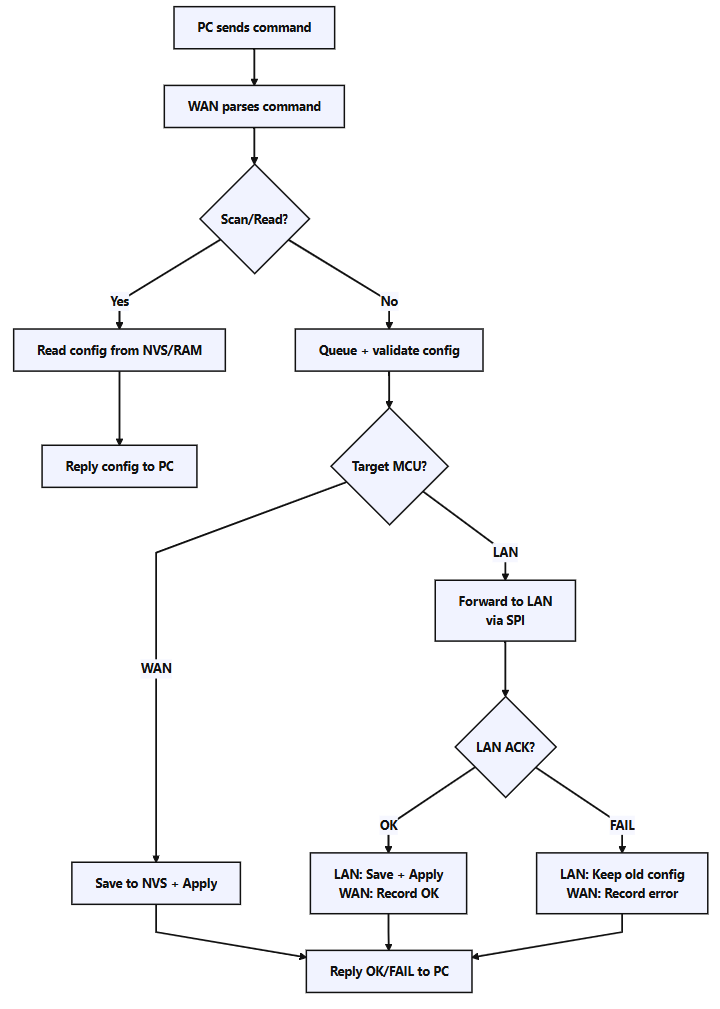
\includegraphics[width=\linewidth]{figures/DATN/design_DCH-CT.png}
                \caption{Lưu đồ giải thuật Data Communication Handler – giao tiếp cấu hình qua USB/UART}
                \label{fig:design_DCH-CT}
            \end{minipage}
        \end{figure}

        \begin{figure}[H]
            \centering
            \begin{minipage}[b]{0.55\textwidth}
                Đối với tác vụ cập nhật cấu hình, WAN-MCU đóng vai trò tiếp nhận mã lệnh tiêu chuẩn, chuỗi JSON từ ứng dụng PC hoặc các gói cấu hình từ Web Portal thông qua HTTP POST. Mọi dữ liệu đầu vào đều được chuyển đổi về định dạng nội bộ, kiểm tra tính hợp lệ và đưa vào hàng đợi xử lý thống nhất.
        
                Tại đây, khối Config Handler sẽ xác thực tham số, lưu vào NVS và lập tức áp dụng vào hệ thống. Trong trường hợp cấu hình thuộc về lớp mạng nội bộ, WAN-MCU sẽ định tuyến gói tin xuống LAN-MCU qua bus SPI. Cuối cùng, Gateway hoàn tất chu trình bằng cách trả về tín hiệu xác nhận OK hoặc FAIL cho người dùng.
            \end{minipage}
            \hfill
            \begin{minipage}[t]{0.4\textwidth}
                \centering
                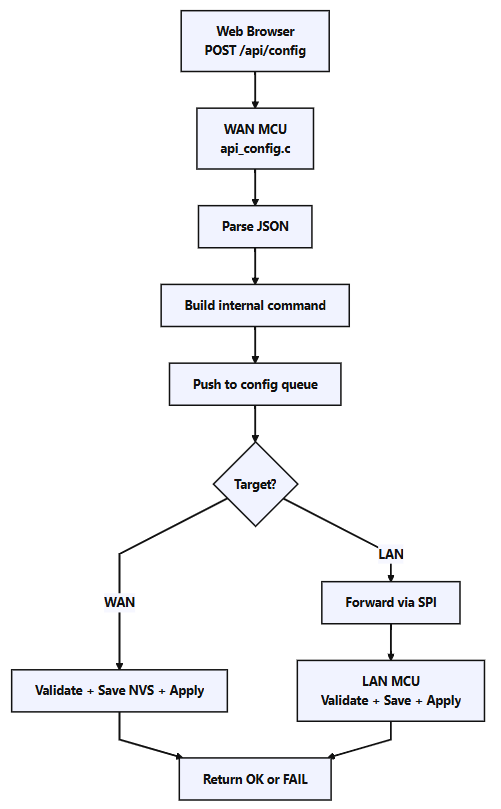
\includegraphics[width=\linewidth]{figures/DATN/design_wcp.png}
                \caption{Lưu đồ giải thuật Config qua Web Config Portal}
                \label{fig:design_wcp}
            \end{minipage}
        \end{figure}

        \begin{figure}[H]
            \begin{minipage}[b]{0.55\textwidth}
                \paragraph{FOTA/Upgrade – cập nhật firmware cho Gateway (LAN cập nhật trước, WAN cập nhật sau)}

                Cơ chế cập nhật Firmware từ xa (FOTA) cho toàn hệ thống được kích hoạt thông qua một lệnh cấu hình chuyên biệt từ Server. Quá trình nâng cấp được thực hiện tuần tự chặt chẽ: LAN-MCU cập nhật trước, sau đó mới đến WAN-MCU.

                Cụ thể, khi tiếp nhận lệnh, WAN-MCU sẽ phân tích, đánh dấu hệ thống chuyển sang chế độ cập nhật và định tuyến lệnh xuống LAN-MCU. Để cung cấp đường truyền tải dữ liệu, WAN-MCU lập tức kích hoạt chế độ điểm truy cập (Wi-Fi AP). Lúc này, LAN-MCU sẽ kết nối vào mạng Wi-Fi nội bộ này để truy cập Internet, từ đó chủ động thực hiện chu trình OTA độc lập, bao gồm tải tệp qua giao thức HTTPS, kiểm tra tính toàn vẹn, ghi vào bộ nhớ flash và khởi động lại.

                Sau khi LAN-MCU hoàn tất cập nhật, nó sẽ gửi tín hiệu handshake nội bộ để thông báo cho WAN-MCU. Ngay khi nhận được tín hiệu đồng bộ này, WAN-MCU bỏ qua bước phản hồi qua lại và lập tức tiến hành chu trình tự cập nhật firmware cho chính mình.

                Kết thúc toàn bộ quy trình, Gateway sẽ gửi bản tin báo cáo trạng thái tổng hợp (OK hoặc FAIL kèm thông tin phiên bản mới) lên Server để xác nhận hoàn tất quá trình nâng cấp hệ thống.
            \end{minipage}
            \hfill
            \begin{minipage}[t]{0.4\textwidth}
                \centering
                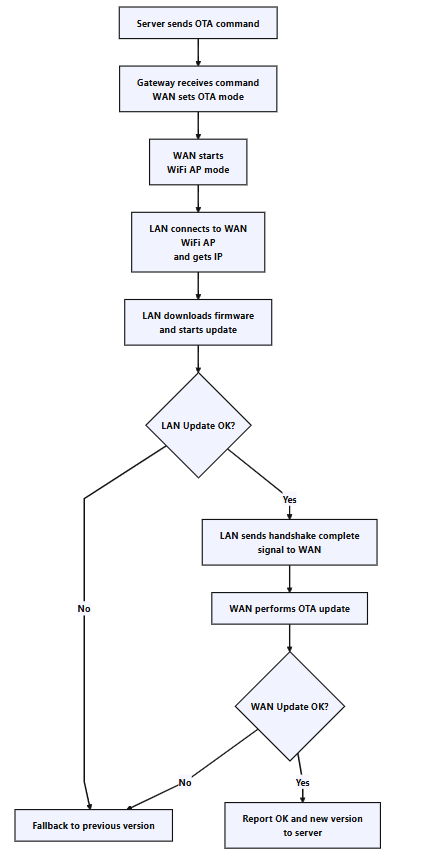
\includegraphics[width=\textwidth]{figures/DATN/design_FOTA.png}
                \caption{Lưu đồ giải thuật FOTA cho Dual-MCU Gateway}
                \label{fig:design_FOTA}
            \end{minipage}
        \end{figure}

    \subsection{Hệ thống cấu hình Module dựa trên JSON (Module Base Setting)}

        Trong kiến trúc ban đầu của gateway, loại module RF gắn vào từng khe phần cứng được coi là cố định tại thời điểm biên dịch. Toàn bộ thông tin đặc thù của module -- cú pháp lệnh AT, chuỗi điều khiển chân GPIO cho reset phần cứng, kiểu giao tiếp và cấu hình tương ứng -- được viết trực tiếp vào mã nguồn firmware. Điều này đặt ra một giới hạn căn bản: mỗi khi hệ thống cần chuyển sang loại module mới, bất kể lý do là thay thế phần cứng hay nâng cấp lên module có tính năng cao hơn, đội kỹ thuật phải sửa firmware, biên dịch lại và nạp lại cho toàn bộ thiết bị đã triển khai.

        Vấn đề này trở nên rõ ràng hơn khi tiến hành phân tích so sánh tám module BLE phổ biến trên thị trường. Phân tích cho thấy một điều nghịch lý: gần như hầu hết chức năng là giống nhau giữa tất cả các module -- đặt tên thiết bị, quét thiết bị lân cận, kết nối, ngắt kết nối, reset phần mềm, reset phần cứng -- nhưng cú pháp lệnh lại khác hoàn toàn. Ví dụ, chức năng đặt tên thiết bị được gọi bằng \texttt{AT+NAME=} trên HC-05, \texttt{AT+BLENAME=} trên module ESP32, và \texttt{AT+GAPDEVNAME=} trên nRF52. Việc chuẩn hóa theo lệnh là không khả thi; nhưng chuẩn hóa theo tên chức năng thì hoàn toàn có thể thực hiện, và đây chính là nền tảng của hệ thống Module Base Setting.

        \paragraph{Ý tưởng triển khai}

        Thay vì hard-code thông tin của từng loại module vào firmware, hệ thống Module Base Setting đưa toàn bộ kiến thức đặc thù của module ra ngoài firmware dưới dạng một file cấu hình JSON có thể cập nhật tại runtime. File JSON mô tả đầy đủ mọi điều firmware cần để vận hành module đó: loại giao tiếp vật lý và các tham số kèm theo, cùng danh sách tất cả chức năng module hỗ trợ. Mỗi chức năng trong danh sách được định nghĩa bởi một tên chuẩn hóa dùng làm khóa tra cứu, một template lệnh AT với placeholder cho tham số động, chuỗi điều khiển GPIO cần thực hiện trước và sau khi gửi lệnh, và giá trị timeout chờ phản hồi.
        
        Ví dụ khi sử dụng module cho BLE, bằng cách này, firmware không còn quan tâm đến việc module đang dùng là STM32WB55 hay nRF52840 -- nó chỉ biết rằng khi cần thực hiện chức năng \texttt{MODULE\_SCAN}, nó sẽ tra cứu tên này trong cấu hình đã nạp và thực thi theo chính xác những gì JSON mô tả. Toàn bộ logic đặc thù của module nằm trong file JSON, không nằm trong firmware. Thay đổi module đồng nghĩa với gửi một file JSON mới, không phải biên dịch lại firmware.
        
        Ba file cấu hình preset đã được chuẩn bị cho giai đoạn kiểm thử: Zigbee E180-ZG120B, BLE STM32WB55 và LoRa Wio-E5. Một file ánh xạ \texttt{stack\_id\_map.json} liên kết định danh khe phần cứng với preset module tương ứng.

        \paragraph{Luồng hoạt động}

        Hệ thống hoạt động theo hai giai đoạn tách biệt: giai đoạn nạp cấu hình module và giai đoạn thực thi lệnh điều khiển. Hình dưới đây mô tả toàn bộ luồng từ khi ứng dụng PC hoặc server gửi JSON config đến khi gateway sẵn sàng thực thi lệnh điều khiển module.

        \begin{figure}[H]
            \centering
            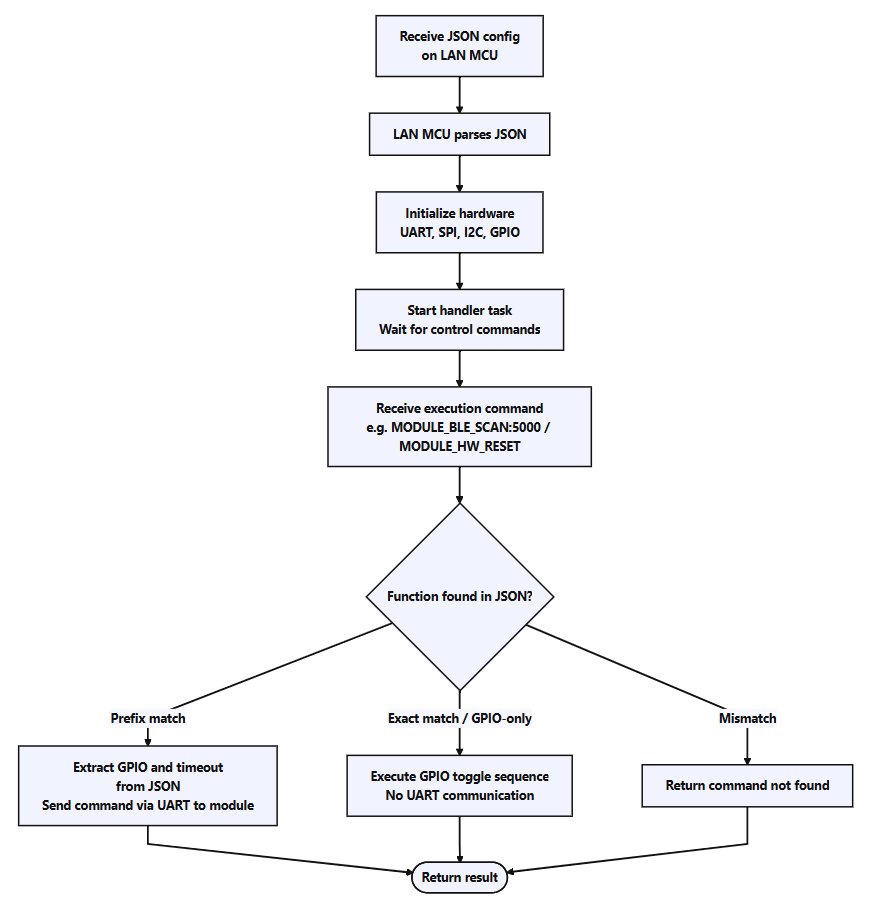
\includegraphics[width=0.6\textwidth]{figures/DATN/design_mbs.png}
            \caption{Luồng hoạt động của Module Base Setting}
            \label{fig:design_mbs}
        \end{figure}

        \paragraph{Kịch bản hoạt động}

        Về kịch bản vận hành, khi có yêu cầu từ người dùng, lệnh điều khiển được truyền xuống WAN-MCU và chuyển tiếp sang LAN-MCU. Tại đây, LAN-MCU phân tích tiền tố để nhận diện chức năng và tra cứu khuôn mẫu (\textit{template}) trong file JSON cấu hình. Nếu là lệnh tĩnh, hệ thống trích xuất trực tiếp chuỗi lệnh thô. Nếu là lệnh động, LAN-MCU sẽ tự động ghép nối tham số từ Server vào khuôn mẫu lệnh. Sau cùng, LAN-MCU kích hoạt trình tự điều khiển GPIO nếu được yêu cầu trong JSON, đẩy lệnh hoàn chỉnh xuống module vật lý và gửi phản hồi trạng thái ngược lên Server.

        Cơ chế linh hoạt này biến Gateway thành một bộ dịch giao thức thông minh. Nó không chỉ giảm tải cho Server khi không cần quản lý các chuỗi lệnh thô phức tạp, mà còn cho phép hệ thống tương thích với các module phần cứng mới chỉ bằng cách cập nhật file JSON cấu hình mà không cần can thiệp vào mã nguồn.

        \begin{figure}[H]
            \centering
            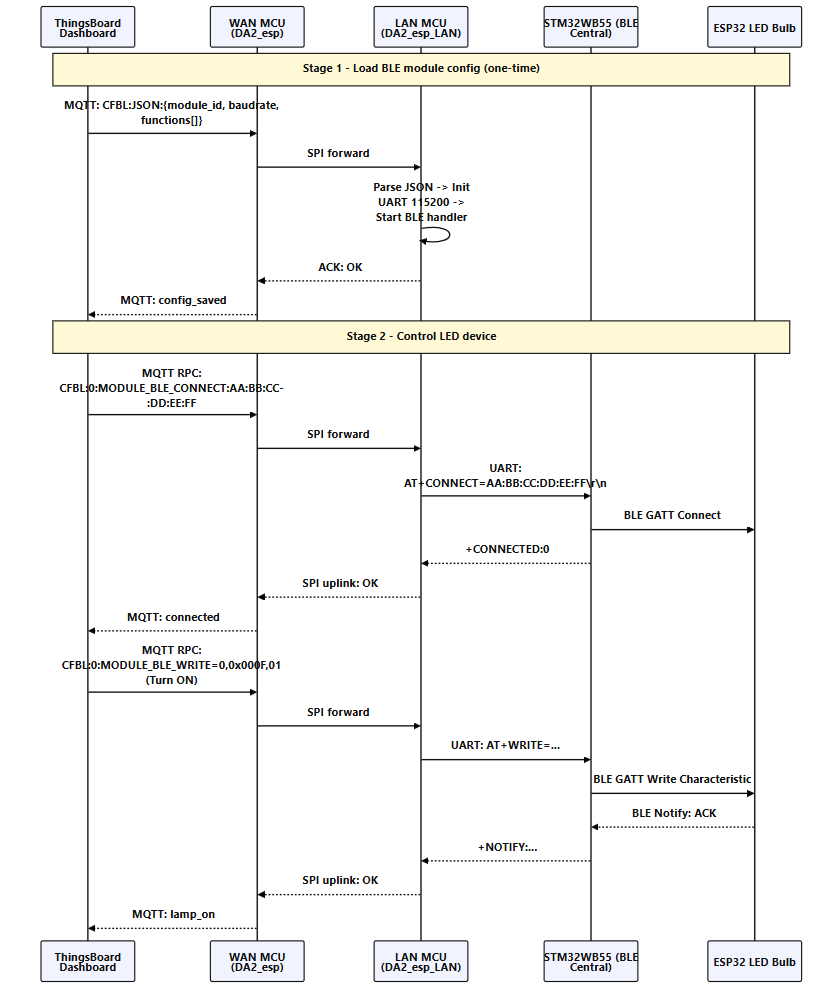
\includegraphics[width=0.55\textwidth]{figures/DATN/design_server-to-bulb.png}
            \caption{Luồng điều khiển end-to-end từ ThingsBoard đến bóng đèn ESP32 qua GW DA2}
            \label{fig:design_server-to-bulb}
        \end{figure}

    \subsection{Xử lý dữ liệu}
        Hệ thống vận hành theo kiến trúc Dual-MCU Master--Slave. LAN-MCU đóng vai trò Master điều phối các giao thức mạng nội bộ, trong khi WAN-MCU đóng vai trò Slave chuyên trách kết nối Cloud. Để tối ưu hóa hiệu suất truyền tải và giảm thiểu tài nguyên xử lý, cơ chế giao tiếp giữa hai MCU được chuyển đổi từ Polling sang Event-driven Handshake thông qua tín hiệu ngắt (Interrupt).
    
        \paragraph{Luồng Uplink: Sensor $\to$ LAN-MCU $\to$ WAN-MCU $\to$ Cloud}
    
            Dữ liệu từ thiết bị đầu cuối được LAN-MCU tiếp nhận, thực hiện hậu xử lý (Validation, Parsing, Normalization) và chuẩn hóa về định dạng khung tin nội bộ.
    
            \begin{itemize}
                \item \textbf{Giao tiếp SPI tin cậy:} Dữ liệu chuyển giao qua kênh SPI được bảo vệ bởi trường CRC và số thứ tự gói (Sequence Number).
                \item \textbf{Bắt tay xác nhận:} WAN-MCU kiểm tra tính toàn vẹn; nếu hợp lệ, phản hồi ACK được gửi lại để LAN-MCU kết thúc giao dịch. Ngược lại, phản hồi NACK sẽ kích hoạt cơ chế Retry.
                \item \textbf{Giao tiếp Cloud/Server:} WAN-MCU thực hiện Publish dữ liệu kèm cơ chế Exponential Backoff để đảm bảo độ tin cậy khi kết nối mạng không ổn định.
            \end{itemize}
            
            \begin{figure}[H]
                \centering
                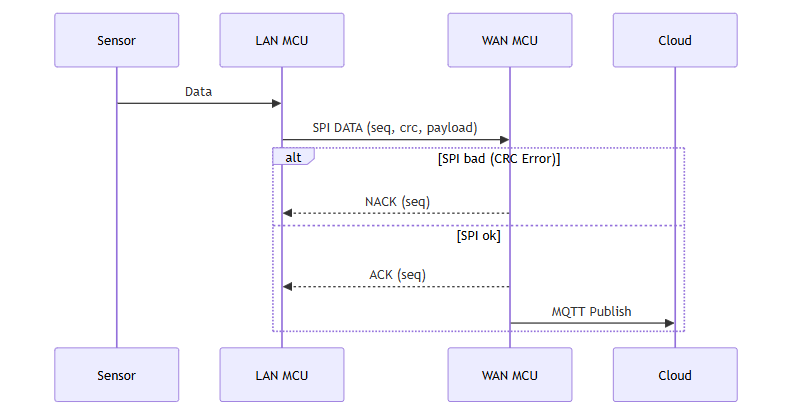
\includegraphics[width=0.55\textwidth]{figures/DATN/sequence_diagram_end-to-end_uplink.png}
                \caption{Sequence diagram: luồng xử lý dữ liệu end-to-end uplink}
            \end{figure}
    
        \paragraph{Luồng Downlink: Cloud $\to$ WAN-MCU $\to$ LAN-MCU $\to$ Sensor}
    
            Khác với cơ chế cũ, luồng Downlink hiện tại được kích hoạt tức thời thông qua tín hiệu phần cứng:
    
            \begin{itemize}
                \item \textbf{Cơ chế GPIO Handshake:} Khi có lệnh từ Cloud, WAN-MCU chủ động kích hoạt (Assert) một chân GPIO Handshake để thông báo dữ liệu đã sẵn sàng.
                \item \textbf{Xử lý ngắt (Interrupt-driven):} LAN-MCU không còn thực hiện truy vấn chu kỳ (Polling). Thay vào đó, việc đọc dữ liệu từ WAN-MCU chỉ được kích hoạt khi LAN-MCU phát hiện cạnh tín hiệu ngắt trên chân Handshake.
                \item \textbf{Thực thi lệnh:} Sau khi nhận gói dữ liệu hợp lệ qua SPI, LAN-MCU điều phối lệnh xuống thiết bị đầu cuối và phản hồi trạng thái (OK/FAIL) ngược lại WAN-MCU để đồng bộ với Cloud.
            \end{itemize}
            
            \begin{figure}[H]
                \centering
                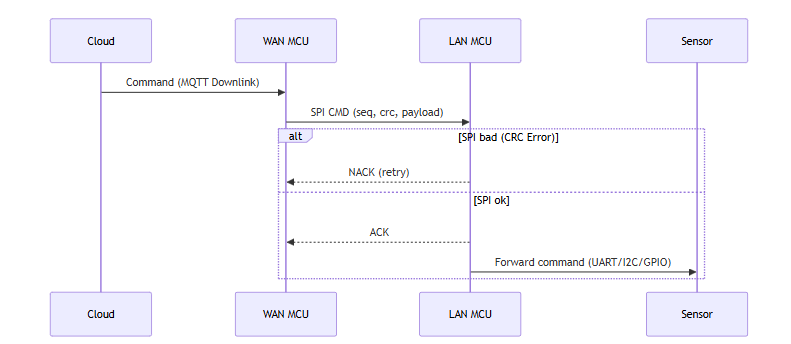
\includegraphics[width=0.6\textwidth]{figures/DATN/sequence_diagram_end-to-end_downlink.png}
                \caption{Sequence diagram: luồng xử lý dữ liệu end-to-end downlink}
            \end{figure}
    
        \paragraph{Cơ chế giao tiếp nội bộ LAN-MCU $\leftrightarrow$ WAN-MCU (SPI Reliability)}
    
            Kênh SPI đóng vai trò xương sống trong truyền tải dữ liệu, vận hành dựa trên các nguyên tắc đảm bảo tính toàn vẹn:
            \begin{itemize}
                \item \textbf{Kiểm tra toàn vẹn (Integrity Check):} Áp dụng thuật toán CRC cho từng khung tin để phát hiện lỗi vật lý trên đường truyền.
                
                \item \textbf{Đồng bộ hóa thứ tự (Sequence Management):} Sử dụng Sequence Number để loại bỏ các gói tin trùng lặp hoặc phát hiện mất gói trong quá trình truyền tải.
                
                \item \textbf{Tối ưu hóa năng lượng và tài nguyên:} Thay thế cơ chế REQ\_DOWNLINK tuần tự bằng cơ chế Async Notify qua GPIO Handshake, giúp LAN-MCU giải phóng chu kỳ CPU cho các tác vụ xử lý cảm biến thời gian thực.
            \end{itemize}
            
            \begin{figure}[H]
                \centering
                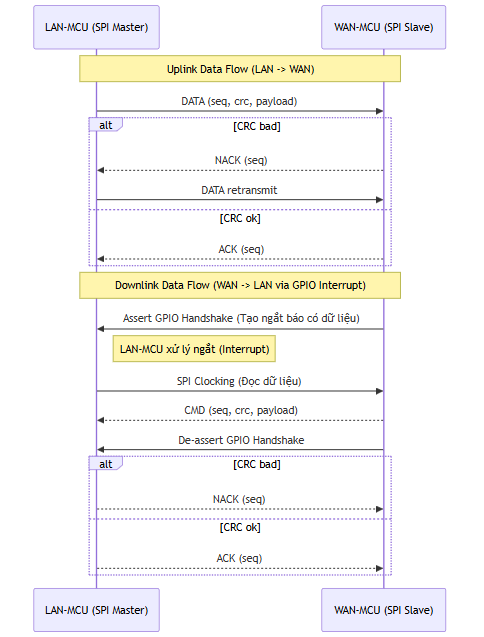
\includegraphics[width=0.48\linewidth]{figures/DATN/sequencediagram_LAN-MCU-WAN-MCU_SPI.png}
                \caption{Sequence diagram: giao tiếp LAN-MCU $\leftrightarrow$ WAN-MCU qua SPI}
                \label{fig:seq_lan_wan_spi}
            \end{figure}
    
            \begin{figure}[H]
                \centering
                \begin{minipage}[b]{0.55\textwidth}
                    \paragraph{Cơ chế cập nhật cấu hình cho Gateway từ App Config PC}
                    Cơ chế cấu hình từ ứng dụng PC cho phép thay đổi tham số mà không cần sửa firmware, trực tiếp tác động đến pipeline dữ liệu như:
                    \begin{itemize}
                        \item Thông số MQTT/HTTP/CoAP, lựa chọn kênh Internet (WiFi, LTE, Ethernet).
                        \item Bật/tắt luồng downlink hoặc định tuyến lệnh.
                        \item Các tham số giao tiếp thuộc LAN, cần chuyển tiếp sang LAN-MCU.
                        \item Cấu hình file JSON cho từng module cắm vào LAN.
                    \end{itemize}
                    Quy trình cập nhật cấu hình gồm 3 thành phần chính: App PC $\rightarrow$ WAN-MCU $\rightarrow$ LAN-MCU tùy trường hợp. WAN-MCU đóng vai trò ``router cấu hình'': nếu cấu hình thuộc WAN thì tự lưu và áp dụng; nếu thuộc LAN thì forward qua SPI và nhận ACK/FAIL từ LAN-MCU.
                \end{minipage}
                \hfill
                \begin{minipage}[t]{0.4\textwidth}
                    \centering
                    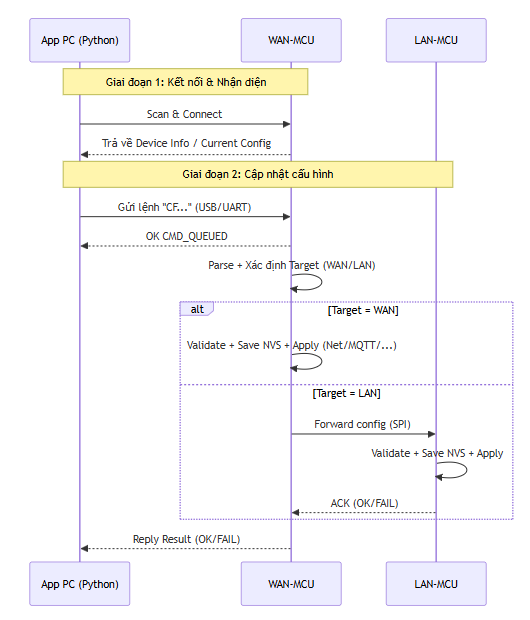
\includegraphics[width=\linewidth]{figures/DATN/sequence_diagram_App-PC_update.png}
                    \caption{Sequence diagram: cập nhật cấu hình từ App PC}
                    \label{fig:seq_app_pc_update}
                \end{minipage}
            \end{figure}
    
            \begin{figure}[H]
                \centering
                \begin{minipage}[b]{0.55\textwidth}
                    \paragraph{Cơ chế cập nhật cấu hình cho Gateway từ Web Config Portal}
                    Cơ chế cấu hình từ Web Config Portal cho phép thay đổi tham số mà không cần sửa firmware, trực tiếp tác động đến pipeline dữ liệu như:
                    \begin{itemize}
                        \item Thông số MQTT/HTTP/CoAP, lựa chọn kênh Internet (WiFi, LTE, Ethernet).
                        \item Bật/tắt luồng downlink hoặc định tuyến lệnh.
                        \item Các tham số giao tiếp thuộc LAN, cần chuyển tiếp sang LAN-MCU.
                        \item Cấu hình file JSON cho từng module cắm vào LAN.
                    \end{itemize}
                    Quy trình cập nhật cấu hình gồm 3 thành phần chính: Web Browser, WAN-MCU, LAN-MCU tùy trường hợp. WAN-MCU đóng vai trò ``router cấu hình'': nếu cấu hình thuộc WAN thì tự lưu và áp dụng; nếu thuộc LAN thì forward qua SPI và nhận ACK/FAIL từ LAN-MCU.
                \end{minipage}
                \hfill
                \begin{minipage}[t]{0.4\textwidth}
                    \centering
                    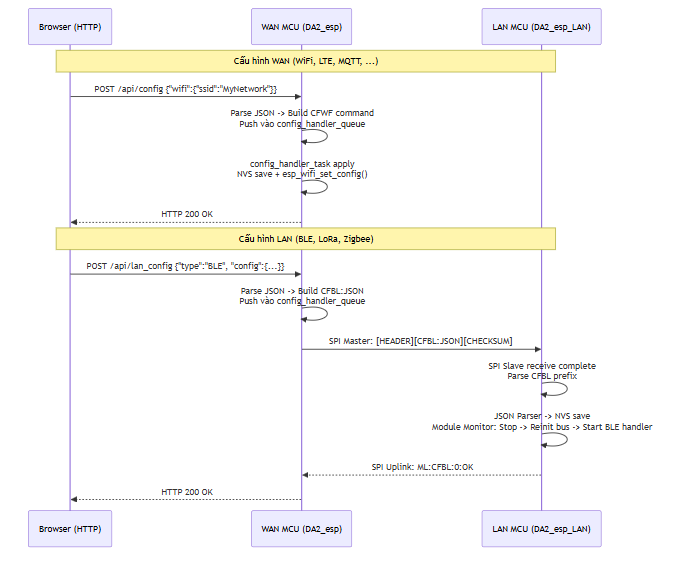
\includegraphics[width=\linewidth]{figures/DATN/sequence_diagram_web-config-portal.png}
                    \caption{Sequence diagram: cập nhật cấu hình từ Web Config Portal}
                    \label{fig:seq_web_config_portal}
                \end{minipage}
            \end{figure}

\newpage